\subsection{Introducci�n}
En esta secci�n se evaluan las pol��ticas de scheduling implementadas, utilizando diversas m�tricas especificadas m�s adelante.

\subsection{Ejercicio 6}
El objetivo de este ejercicio es programar un tipo de tarea \textbf{TaskBatch}, que durante \textit{total\_cpu} ciclos, realize \textit{cant\_bloqueos} llamadas bloqueantes, 
en momentos elegidos pseudoaleatoriamente. La implementaci�n es bastante directa, con la semilla del generador de n�meros pseudoaleatorios inicializada con la fecha del sistema
al momento de ejecutar la funci�n. Las llamadas bloqueantes se lanzan si \textit{rand()} devuelve un n�mero impar. Para asegurarnos de que se ejecuten 
las \textit{cant\_bloqueos} llamadas bloqueantes antes de que se terminen los \textit{total\_cpu} ciclos, creamos procesos cuya cantidad de llamadas bloqueantes fuese
menor o igual a la mitad de los ciclos totales de CPU.

Para m�s detalles, consultar la implementaci�n en \textit{tasks.cpp}.

\subsection{Ejercicio 7}

En este ejercicio debemos elegir 2 m�tricas diferentes y testear un lote de tareas \textbf{TaskBatch}, todas ellas con igual uso de CPU pero con diversas
cantidades de bloqueos. El lote de tareas utilizado es el \textit{lote3.tsk}.

Las m�tricas que elegimos fueron:
\begin{itemize}
 \item Turnaround
 \item Waiting Time 
\end{itemize}

Definidas en [Sil1] como:
\newline

\textbf{Turnaround}: Es el intervalo de tiempo entre el momento en que el proceso comienza a ejecutarse por primera vez, hasta el momento en que
el mismo termina. Es decir, es la suma de los per�odos usados en esperar datos de memoria, en estar encolado en la ``ready queue'', ejecutandose en 
la CPU, y haciendo E/S.


\textbf{Waiting Time}: Es el tiempo que un proceso se pasa encolado en la ``ready queue''.
\newline
\newline
Elegimos estas m�tricas ya que, con el Turnaround, tenemos una visi�n global de c�mo se comportan los procesos, mientras que con el Waiting Time
podemos observar c�mo un hecho m�s puntual, el tiempo que los procesos pasan encolados, impacta en el tiempo de ejecuci�n total del proceso.
\newline
\newline
Para calcular el desv�o standard utilizamos la f�rmula de [WikSD]
\newline
\newline
A continuaci�n se pueden observar los resultados de la experimentaci�n:
\newline
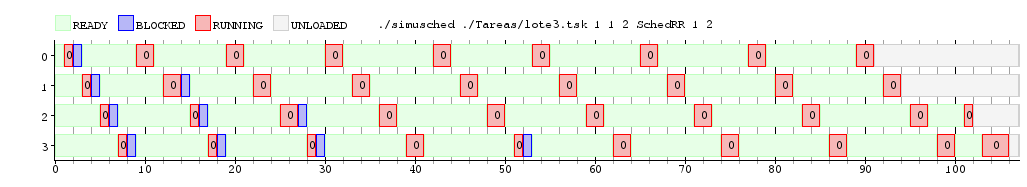
\includegraphics[width=1\textwidth]{./Graficos/ej7_1core_q2.png}
\begin{center}
 \textit{1 core, quantum = 2}.
\end{center}
~\\
\newline
Turnaround:  \hspace{7cm}  Waiting Time:

$P_{0}$: 59  \hspace{8cm}    $P_{0}$: 42

$P_{1}$: 81  \hspace{8cm}    $P_{1}$: 67

$P_{2}$: 67  \hspace{8cm}    $P_{2}$: 55

$P_{3}$: 86  \hspace{8cm}    $P_{3}$: 75


Promedio: 73,25 \hspace{6,5cm}   Promedio: 59,75


DS: 10,78           \hspace{7,4cm}    DS: 12,47
%----------------------------------------------------------------------------------------------

~\\
\newline
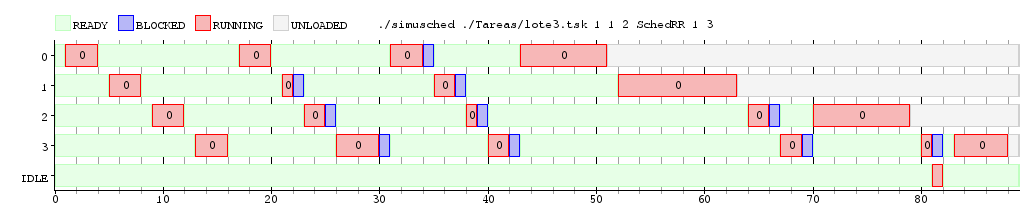
\includegraphics[width=1\textwidth]{./Graficos/ej7_1core_q3.png}
\begin{center}
 \textit{1 core, quantum = 3}.
\end{center}
~\\
\newline
Turnaround:  \hspace{7cm}  Waiting Time:

$P_{0}$:   \hspace{8cm}    $P_{0}$: 

$P_{1}$:   \hspace{8cm}    $P_{1}$: 

$P_{2}$:   \hspace{8cm}    $P_{2}$: 

$P_{3}$:   \hspace{8cm}    $P_{3}$: 


Promedio:    \hspace{6,6cm}    Promedio: 


DS:          \hspace{7,4cm}    DS: 
~\\
\newline





\subsection{Ejercicio 8}

\subsection{Ejercicio 9}

\subsection{Ejercicio 10}